\documentclass[12pt,a4paper,oneside]{article}

\usepackage[utf8]{inputenc}
\usepackage[portuguese]{babel}
\usepackage[T1]{fontenc}
\usepackage{amsmath}
\usepackage{amsfonts}
\usepackage{amssymb}
\usepackage{graphicx}

\usepackage{xcolor}
% Definindo novas cores
\definecolor{verde}{rgb}{0.25,0.5,0.35}
\definecolor{jpurple}{rgb}{0.5,0,0.35}
% Configurando layout para mostrar codigos Java
\usepackage{listings}
\lstset{
  language=Java,
  basicstyle=\ttfamily\small, 
  keywordstyle=\color{jpurple}\bfseries,
  stringstyle=\color{red},
  commentstyle=\color{verde},
  morecomment=[s][\color{blue}]{/**}{*/},
  extendedchars=true, 
  showspaces=false, 
  showstringspaces=false, 
  numbers=left,
  numberstyle=\tiny,
  breaklines=true, 
  backgroundcolor=\color{cyan!10}, 
  breakautoindent=true, 
  captionpos=b,
  xleftmargin=0pt,
  tabsize=4,
  escapeinside=||
}

\author{\\Universidade Federal de Jataí (UFJ)\\Bacharelado em Ciência da Computação \\Inteligência Artificial \\Esdras Lins Bispo Jr.}

\title{\sc \huge Primeira Prova}

\begin{document}

\maketitle

{\bf ORIENTAÇÕES PARA A RESOLUÇÃO}

\begin{itemize}
	\item A avaliação é individual, sem consulta;
	\item A pontuação máxima desta avaliação é 10,0 (dez) pontos, sendo uma das 04 (quatro) componentes que formarão a média final da disciplina: duas provas, um projeto e exercícios;
	\item A média final será calculada pela média ponderada das quatro supraditas notas [em que a primeira prova tem peso 40 (quarenta), a segunda prova tem peso 30 (trinta), o projeto tem peso 30 (trinta) e os exercícios-bônus são adicionados à media final];
	\item O somatório da pontuação de todas as questões desta avaliação é 11,0 (onze) pontos. Isto é um sinônimo de tolerância na correção. Se você por acaso perder 1,5 (um e meio), sua nota será 9,5 (nove e meio);
	\item O conteúdo exigido compreende os seguintes pontos apresentados no Plano de Ensino da disciplina: (1) Introdução à Inteligência Artificial, (2) Agentes Inteligentes, (3) Resolução de Problemas por meio de Busca, (5) Redes Neurais Artificiais, e  (6) Computação Natural.
\end{itemize}

\begin{center}
	\fbox{\large Nome: \hspace{10cm}}
	\fbox{\large Assinatura: \hspace{9cm}}
\end{center}

\newpage

\begin{enumerate}


	\item[] \colorbox{black}{
		\color{white}Todas as questões necessitam não apenas
	}\\ 
	\colorbox{black}{
		\color{white} serem respondidas, mas também justificadas.
	}

	\item (2,0 pt) {\bf [Russel 1.11 Adaptado]} ``Sem dúvida, os computadores não podem ser inteligentes - eles só podem fazer o que seus programadores determinam''. Esta última afirmação é verdadeira e implica a primeira? Justifique sua resposta baseado na discussão sobre as várias definições de Inteligência Artificial.
			
	\item (2,0 pt) {\bf [ENADE 2008]} Julgue os itens a seguir, relativos a métodos de busca com informação (busca heurística) e sem informação (busca cega), aplicados a problemas em que todas as ações têm o mesmo custo, o grafo de busca tem fator de ramificação finito e as ações não retornam a estados já visitados.
	
	\begin{enumerate}
		\item[] I - A primeira solução encontrada pela estratégia de busca em largura é a solução ótima.
		\item[] II - A primeira solução encontrada pela estratégia de busca em profundidade é a solução ótima.
		\item[] III - As estratégias de busca com informação usam funções heurísticas que, quando bem definidas, permitem
		melhorar a eficiência da busca.
		\item[] IV - A estratégia de busca gulosa é eficiente porque expande apenas os nós que estão no caminho da
		solução.
	\end{enumerate}
	
	Estão certos apenas os itens:
	
	\begin{enumerate}
		\item I e II.
		\item I e III.
		\item I e IV.
		\item II e IV.
		\item III e IV.
	\end{enumerate}
	
	 \item (2,0 pt) {\bf [Russel 2.6 Adaptado]} Pode haver mais de um programa de agente que implemente uma
	dada função de agente? Dê um exemplo ou mostre por que não é
	possível.
	
	\item (2,0 pt)  Explique por quê o Perceptron pode executar as funções lógicas AND, OR e NOT, mas não resolve o OU-EXCLUSIVO (XOR).
	
	\item (3,0 pt) O grafo abaixo mostra a ligação entre 5 cidades e as respectivas distâncias em quilômetros:
	
	\begin{center}
		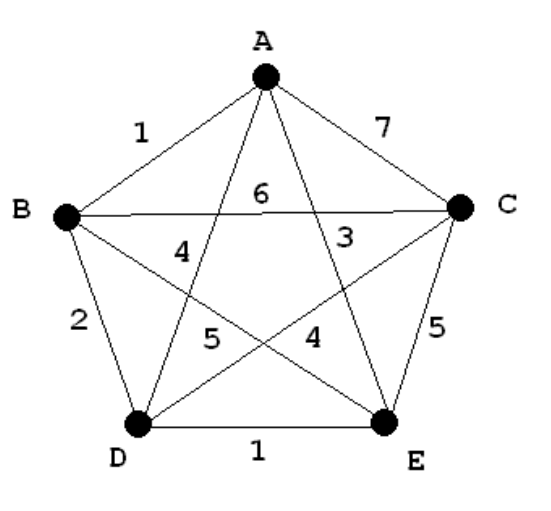
\includegraphics[width=5cm]{images/fig02.png}
	\end{center}
	
	Tem-se um problema em que é necessário passar por todas as cidades, apenas uma vez. O objetivo é encontrar uma rota de menor custo usando um algoritmo genético.
	
	\begin{enumerate}
		\item (0,5 pt) Proponha uma maneira de codificar os cromossomos.
		\item (0,5 pt) Defina uma função de aptidão para avaliar a qualidade dos cromossomos.
		\item (0,5 pt) Realize o cruzamento entre os cromossomos.
		\item (0,5 pt) Aplique uma mutação em um gene dos cromossomos.
		\item (0,5 pt) Aplique a função de aptidão nos descendentes gerados verificando se a solução encontrada é melhor ou não.
	\end{enumerate}
\end{enumerate}
\end{document}